\chapter{Project Overview}
\minitoc
\newpage

% \setcounter{secnumdepth}{0} % Set the section counter to 0 so next section is not counted in toc
% % ----------------------- Introduction ----------------------- %
% \section{Introduction}
% \lipsum[2][1-5]

\setcounter{secnumdepth}{2} % Resume counting the sections for the toc with a depth of 2 (Sections and sub-sections)
% ----------------------------------- SECTIONS (v) ----------------------------------- %
% ----------------------- General framework of the internship ----------------------- %
\section{General framework of the internship}
% \lipsum[2]
This project was conducted as part of the requirements for obtaining a bachelor’s degree in Computer Science at the Higher Institute of Technological Studies of Nabeul (ISETN). The project was executed at the Information Promotion Agency (IPA) over a period of three months, starting from the 26th of February 2023 to the 31st of May 2023. The primary objective of the project was to simplify and enhance the usability of the i Competency Dictionary (iCD) toolset, a comprehensive framework for understanding and developing IT skills. The project involved the development of a user-friendly web or mobile application, the translation of complex iCD data into a more accessible format, and the automation of relevant skills and tasks fetching process. The project aimed to adhere to modern software development principles and improve the scalability of the iCD toolset for effective IT recruitment and skill development.


% ----------------------- Company overview ----------------------- %
\section{Introduction to the Hosting Organization}
This section introduces the host company {\bf Information Promotion Agency} as well as the services it offers.

\subsection{About IPA}
The Information-technology Promotion Agency (IPA) is a government-affiliated organization in Japan. It is dedicated to advancing the development and widespread adoption of information and communication technologies (ICT) across various sectors, including businesses, government agencies, and individuals.
\begin{figure}[H]
    \centering
    \makebox[\textwidth]{
\includegraphics[width=12cm]{src/assets/logos/IPA_LOGO.png}}
    \caption{Information Promotion Agency Logo}
    \label{fig:logo-of-IPA}
\end{figure}

\subsection{IPA's services}
\subsubsection*{\underline{Information Security Enhancement}}
One of the primary services of IPA is enhancing information security. They provide guidance and support to various sectors to help them adopt and leverage ICT effectively. This includes assisting the Japanese government in the formulation and implementation of ICT policies and strategies, fostering innovation in the ICT industry, and enhancing cybersecurity measures.

\subsubsection*{\underline{Professional Development and Talent Nurturing}}
IPA is involved in conducting national IT examinations and other initiatives aimed at developing skilled ICT professionals. They are committed to nurturing talents and professionals for the digital age, which is crucial for the advancement of the ICT sector in Japan.

\subsubsection*{\underline{Digital Transformation Enablement}}
IPA plays a significant role in enabling digital transformations in industries and society. They drive various IT initiatives to create a super-smart society, which involves fostering innovation in the ICT industry, developing new technologies, and promoting their adoption across various sectors.

% \begin{figure}[H]
%     \centering
%     \makebox[\textwidth]{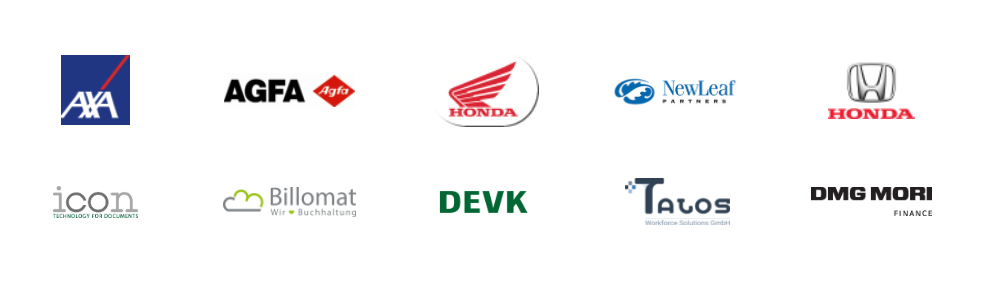
\includegraphics[width=\linewidth]{src/assets/images/selection-of-clients.JPG}}
%     \caption{Selection of MyAwesomeGroup clients}
%     \label{fig:selection-of-clients}
% \end{figure}

% ----------------------- Stating the problem ----------------------- %
\section{Project Context}
The i Competency Dictionary (iCD) project is an initiative launched by IPA to improve IT human resource development and skills enhancement in Japan. The iCD is a comprehensive database of tasks and skills related to the field of IT engineering, designed to help both companies/organizations and individuals enhance their ability to execute tasks and reach their goals by improving their skills. The iCD comprises two main components: the Task Dictionary and the Skill Dictionary. The Task Dictionary defines internal tasks performed by IT engineers, while the Skill Dictionary defines the skills required to execute those tasks.

\newpage
\subsection{iCD Structure}
The iCD is composed of two main components: the Task Dictionary and the Skill Dictionary. The Task Dictionary provides a comprehensive list of tasks in IT business, organized into four layers, including three task layers and an Assessment Items layer. The Skill Dictionary, on the other hand, offers a detailed list of IT skills required to perform those tasks, divided into four layers, including three skill layers and a BOK (Body of Knowledge) layer.

\begin{figure}[H]
    \centering
    \makebox[\textwidth]{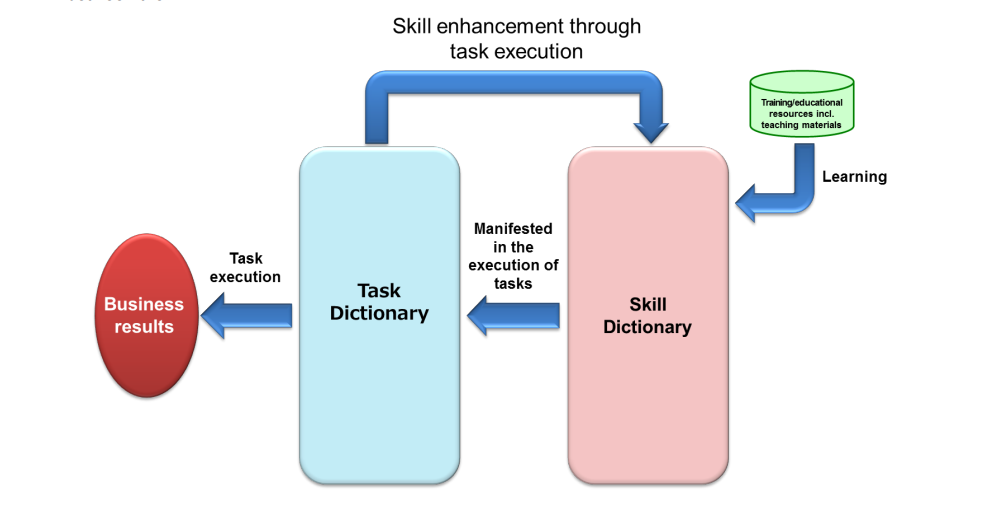
\includegraphics[width=\linewidth]{src/assets/images/iCDRelationship.PNG}}
    \caption{ Relationship between Task execution and Dictionaries}
    \label{fig:task_dictionaries_Relationship}
\end{figure}

\subsection{iCD Contents}
The iCD is comprised of several components, including:

\begin{enumerate}
    \item Task List
    \item Task Dictionary Chart
    \item Task Profile
    \item Task Profile X Task Corresponding table
    \item Skill List
    \item Skill Dictionary Chart
    \item Job List
    \item Job X Skill Corresponding table
    \item ITEE X Skill Corresponding table
    \item Task X Skill corresponding table (Second layer)
    \item Task X Skill corresponding table (Third layer)
\end{enumerate}

\begin{figure}[H]
    \centering
    \makebox[\textwidth]{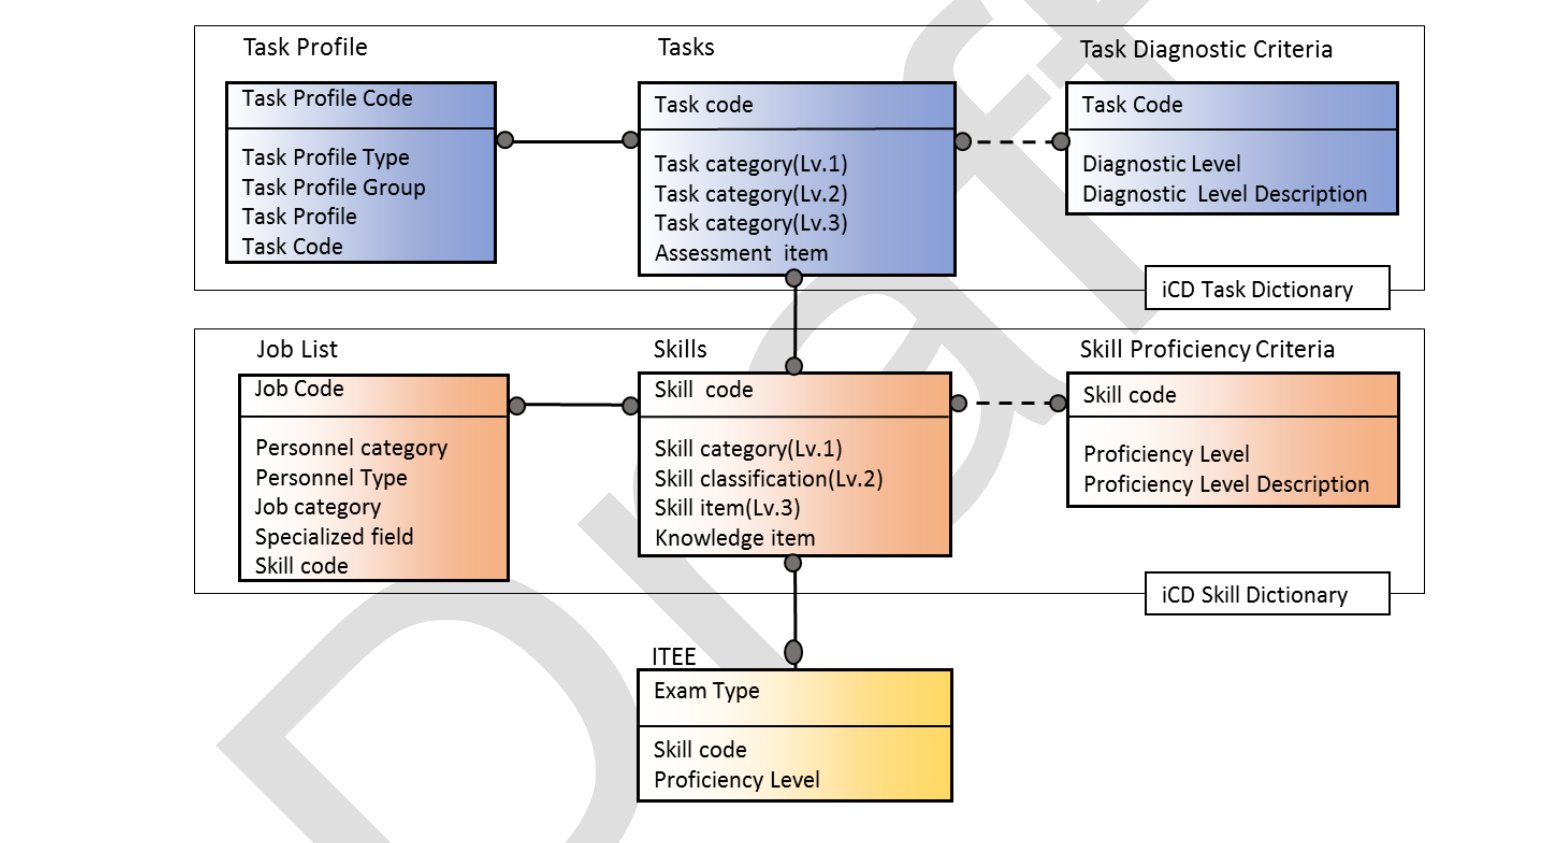
\includegraphics[width=\linewidth]{src/assets/images/iCDERDiagram.PNG}}
    \caption{ i Competency Dictionary (iCD) ER Diagram }
    \label{fig:iCD_ER_Diagram}
\end{figure}

\begin{itemize}
    \renewcommand\labelitemi{-}
    \item These components provide a comprehensive framework for IT competencies, enabling organizations to assess and develop the competencies of their employees in the IT service industry, IT user organizations, and embedded software development.
    \item In conclusion, the i Competency Dictionary (iCD) project aims to improve IT human resource development and skills enhancement in Japan by providing a comprehensive database of tasks and skills related to the field of IT engineering. By understanding the structure, objectives, applications, benefits, implementation status, supplementary contents, and update process of the iCD, readers will gain valuable insights into the importance of this project in the context of IT human resource development and skills enhancement in Japan and globally.
\end{itemize}

\newpage
\subsection{Task Dictionary}
The "Task Dictionary" is intended to be used and applied by companies and organizations in order to
determine internal tasks in line with their business strategy or business plan. The structure of the dictionary
assumes a wide range of corporate activities so that companies with any kind of business model can use
and apply it.
It includes "Task Dictionary Chart" and "Task Profiles" and is expected to be used for reference when
internal tasks are formulated.

\begin{figure}[H]
    \centering
    \makebox[\textwidth]{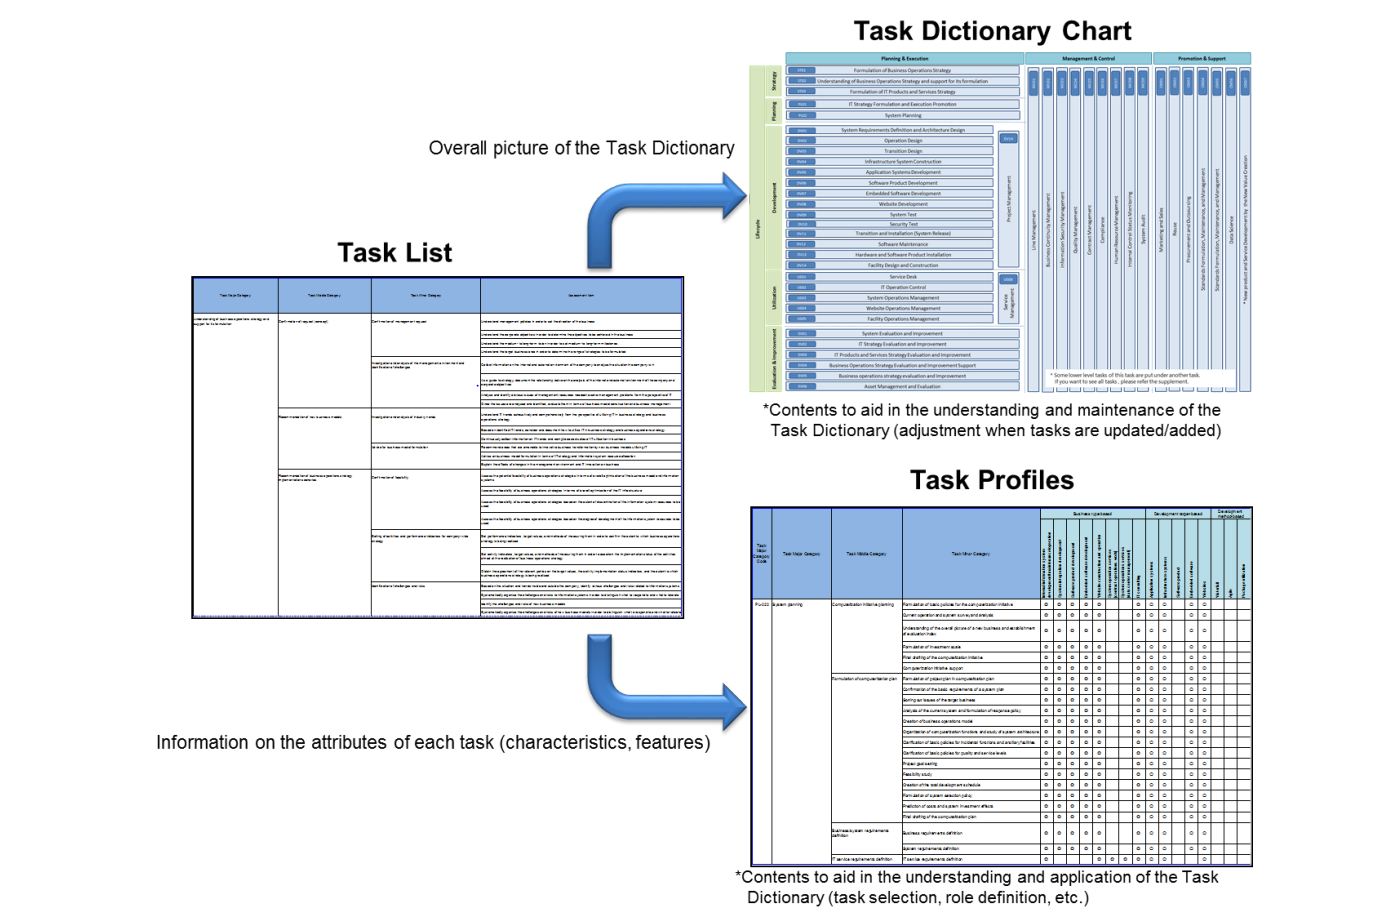
\includegraphics[width=\linewidth]{src/assets/images/taskDictionaryStructure.PNG}}
    \caption{ Structure of the Task Dictionary }
    \label{fig:task_Dictionary_Structure}
\end{figure}

\begin{enumerate}
\item Task List \\
In discussions about IT human resource development, companies and organizations use their corporate strategy or business plan to identify key tasks from the Task List for defining personnel roles. 
% \newpage
These tasks, stratified into Major, Middle, and Minor Categories, are composed of assessment items and fall into three groups:
\begin{itemize}
\renewcommand\labelitemi{-}
\item Tasks for the "planning/execution" of a business lifecycle using IT, including strategy, planning, development, use and application, and evaluation/improvement.
\newpage
\item Tasks that "manage/control" to ensure efficient and effective execution.
\item Tasks that "promote/support" the implementation of other tasks.
\end{itemize}
Each task can be identified by its unique task code. For each Minor Category, "Assessment Items" are provided as examples of specific implementations, which can be used as references when deciding whether to execute a task.

\item Task Dictionary Chart \\
The Task Dictionary Chart represents a task structure composed of the business lifecycle (strategy,
planning, development, use and application, evaluation/improvement) and the four task groups:
"Planning/Execution," "Management/Control," "Promotion/Support", and “Other tasks”. By obtaining a
bird's-eye view of the entire Task Dictionary on the Major Category level, users are expected to apply it for
the formulation of their internal tasks.
\begin{figure}[H]
    \centering
    \makebox[\textwidth]{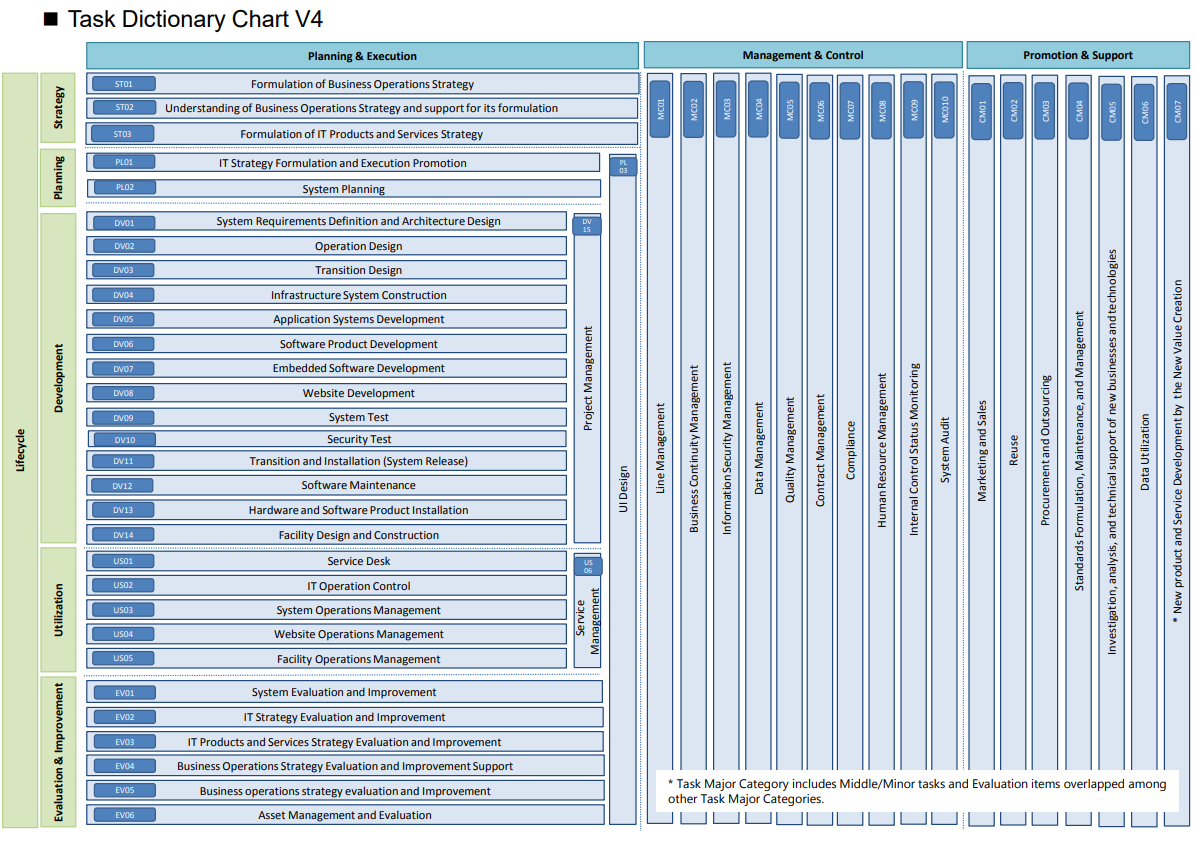
\includegraphics[width=\linewidth]{src/assets/images/taskDictionaryChart.PNG}}
    \caption{ Task Dictionary Chart }
    \label{fig:task_Dictionary_Chart}
\end{figure}

\newpage
\item Task Profiles \\
"Task Profiles" serve as a reference to understand tasks when selecting from the Task List for internal task formulation. They are provided in two forms: the "List of Task Profiles" (detailing each task profile) and the "Task Profile × Task Correspondence Table."

Task profiles are categorized based on features and characteristics such as corresponding business/function or development target:
\begin{enumerate}
    \item Business Type-Based: Task sets necessary depending on the organization's position (user, vendor) or business category, like internal information system development/maintenance/operations, software product development, and system operation services.
    \item Development Target-Based: Task sets needed depending on the type of target for development, construction, maintenance, or operation, such as application systems, infrastructure systems, and embedded software.
    \item Development Method-Based: Task sets required depending on the type of development methods or means such as Waterfall, Agile, etc.
    \item New Business-Based: Task sets essential for personnel taking on new businesses and functions like cloud business, data science, information security, etc.
    \item Role-Based: Task sets that can serve as reference information for companies and organizations when determining their own roles.
\end{enumerate}
Task Profiles are assigned based on case studies from various training activities for IT professionals. However, they don't consider the individual circumstances and characteristics of companies and organizations. Therefore, when using Task Profiles, organizations should not solely rely on this information to determine essential tasks, but also consider their own business types and processes.

\end{enumerate}

\newpage
\subsection{Skill Dictionary}
The "Skill Dictionary" is structured so that it can be used and applied independently to focus on skills and
boost training activities. It is expected to be used in the combination with various other qualifications and
certification examinations including Information Technology Engineers Examination, and school-related or
educational providers' curricula.

The Skill Dictionary is divided into four categories based on skill characteristics: "Methodology",
"Technology”, "Related Knowledge”, and "IT Human Skills”.
Methodology, Technology, and Related Knowledge summarize knowledge items with the Skill Standards,
CCSF (Supplement), and other major Bodies of Knowledges as a reference base.
IT Human Skills serves as a reference model for companies and organizations assigning human skills
essential to the execution of IT-related tasks based on their business type, organizational climate or
environment, etc.

\begin{figure}[H]
    \centering
    \makebox[\textwidth]{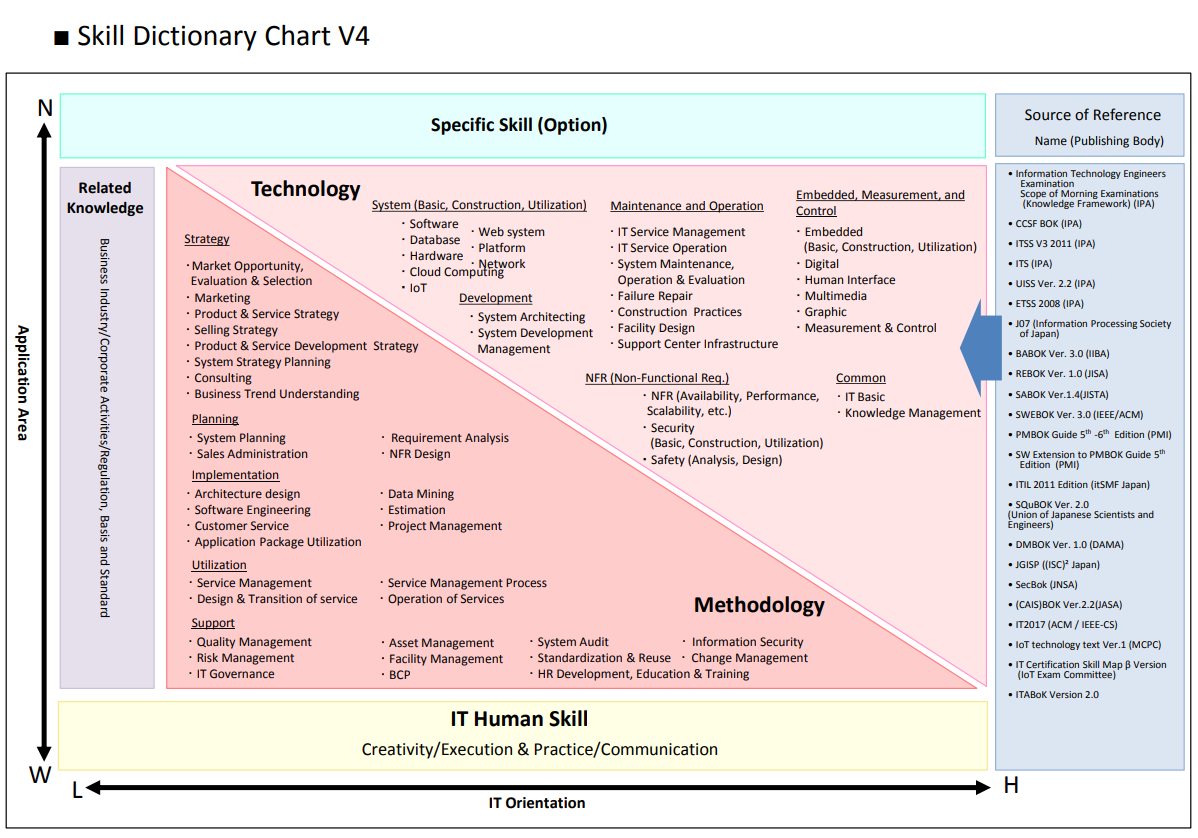
\includegraphics[width=\linewidth]{src/assets/images/SkillDictionaryDiagram.PNG}}
    \caption{  Diagram of the Structure of the Skill Dictionary }
    \label{fig:skill_Dictionary_Diagram}
\end{figure}

\newpage
Using the examples of knowledge items and main Bodies of Knowledge in the Skill Standards and
Information Technology Engineers Examination as a reference base, the Skill Dictionary summarizes and
catalogs skills and knowledge items essential to the execution of IT-related tasks.

\subsection{Objectives of the iCD}
The primary objectives of the iCD are:

\begin{itemize}
    \item To consolidate IT skills standards (ITSS, UISS, ETSS) to create a comprehensive, unified framework
    \item To regularly update the iCD based on user feedback, global IT trends, ITEE alignment, and other global standards and BOKs available in Japanese
    \item To provide organizations with a tool to assess and develop the competencies of their employees in the IT service industry, IT user organizations, and embedded software development
\end{itemize}


\subsection{Applications of the iCD}
The iCD can be utilized by various stakeholders in different ways, such as:

\begin{itemize}
    \item Companies using the iCD for workforce planning, skill gap analysis, and training program development
    \item Educational institutions, like university IT departments and IT engineering schools, using the Skill Dictionary to establish syllabi or curricula
    \item IT professionals leveraging the iCD to identify career paths and skill requirements for their desired roles
\end{itemize}

While the iCD toolset serves a broad range of stakeholders, for the purpose of this project, we primarily focus on its application within companies for workforce planning, skill gap analysis, and training program development. This focus is driven by the project's time constraints and our supervisor's instructions. By concentrating on this specific application, we aim to deliver a solution that effectively addresses the needs of HR managers and recruiters in IT companies. This focus also allows us to delve deeper into the complexities and nuances of this application, thereby ensuring a more thorough and detailed solution. Future iterations of the project may expand to cover other applications of the iCD toolset.

\begin{figure}[H]
    \centering
    \makebox[\textwidth]{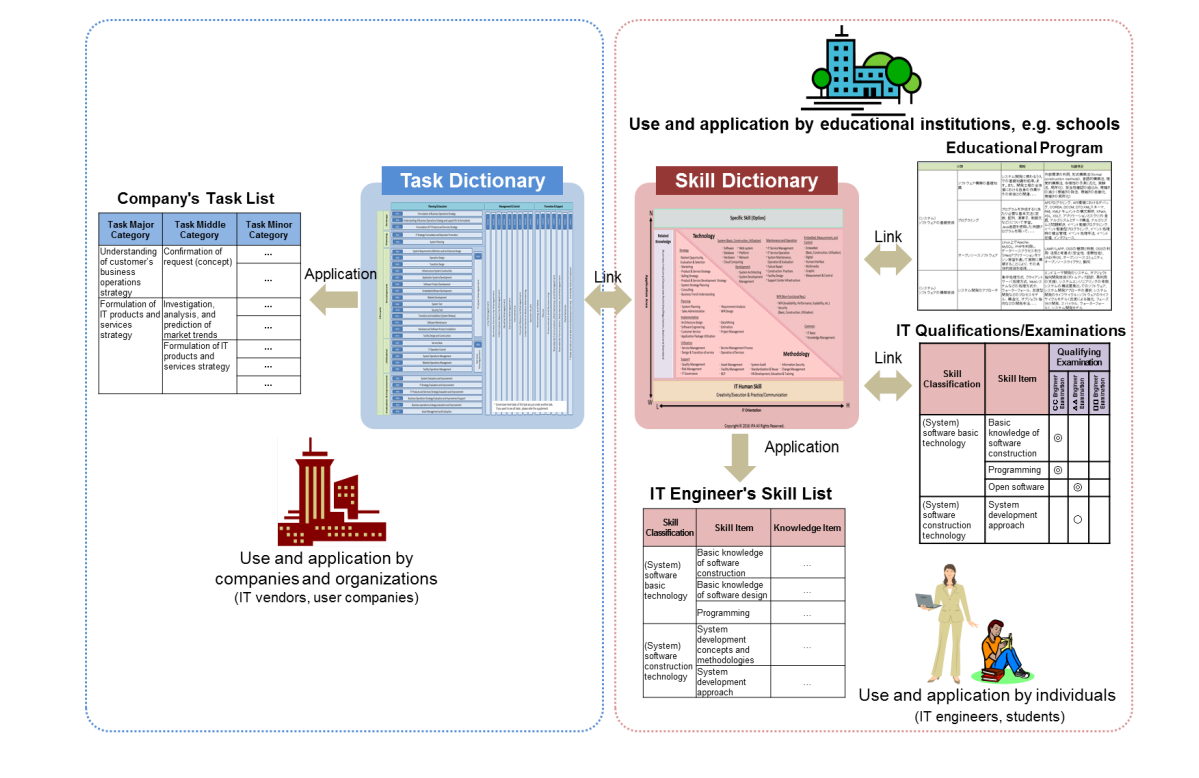
\includegraphics[width=\linewidth]{src/assets/images/iCDformsOfUse.PNG}}
    \caption{Forms of Use and Application of the i Competency Dictionary}
    \label{fig:iCD_Forms_Of_Use}
\end{figure}

\subsection{Benefits of the iCDe}
Some of the key benefits of implementing the iCD are:
\begin{itemize}
    \item Enhanced workforce adaptability and productivity
    \item More effective and targeted training programs
    \item Better alignment between education and industry requirements
    \item Improved career development and job satisfaction for IT professionals
\end{itemize}


\subsection{iCD Implementation Status}
The iCD has seen widespread adoption, with approximately 1,000 organizations obtaining user company certification as of September 2017. Notably, HITACHI Ltd uses the iCD for level checks for around 20,000 employees. In addition to its applications in industry, the iCD has also been implemented in academia, such as university IT departments and IT engineering schools. The iCD's popularity has grown globally since the release of the English version in 2015, with 24 countries adopting it, including regions in Europe, the Middle East, Asia, and North/South America.

\subsection{iCD Supplement}
- The Supplementary contents of the iCD Task Dictionary include specific, urgent, or special task requests from Japanese companies. These contents are not linked to skills and are not included in the English translation of the iCD for overseas use. The Supplementary contents cover tasks related to Marketing, General Affairs/Personnel Affairs/Accounting, Education, Call Centers, and IoT System Service Lifecycle.

- By incorporating these sub-elements, you will provide a comprehensive understanding of the iCD's background, structure, objectives, applications, benefits, implementation status, and supplementary contents, which will help readers appreciate the importance of the project in the context of IT human resource development and skills enhancement.


\subsection{iCD Update Process}

\begin{itemize}
    \item Feedback from users and stakeholders: By incorporating their voices and opinions, the iCD can adapt to changing needs and remain a valuable resource for organizations.
    \item Global IT trends: The iCD collaborates with various global partners to capture and incorporate the latest IT trends and best practices.
    \item Consistency with ITEE updates: Ensuring consistency between the iCD and the ITEE is crucial for maintaining the iCD as a reliable reference for IT professionals and organizations preparing for the ITEE.
    \item Updates of other global standards and BOKs available in Japanese: The iCD updates are aligned with other global standards and BOKs to ensure consistency and provide a comprehensive understanding of the IT competencies required in the current business environment.
\end{itemize}



% ----------------------- Assessment of the case ----------------------- %
\newpage
\section{Problems and Motivations}
In this section, we delve into the core issues that motivated the inception of this project and the proposed solution to address these challenges. The complexities of the IT landscape and the difficulties faced by organizations and individuals in identifying and developing necessary IT competencies form the crux of the problem. The iCD toolset, despite its comprehensive nature, presents its own set of challenges that hinder its effective utilization. Our proposed solution aims to tackle these issues head-on, by simplifying the iCD toolset and making it more accessible and user-friendly through an integrated web application. The following subsections provide a detailed description of the problem and the proposed solution.

\subsection{Problem Description}
\begin{itemize}
    \renewcommand\labelitemi{-}
    \item The rapid evolution of the IT landscape has led to a growing demand for skilled IT professionals with the ability to adapt to new technologies and challenges. However, it can be difficult for both organizations and individuals to identify the specific competencies required to excel in the field. Traditional methods for assessing IT skills may be insufficient or outdated, and there may be a lack of comprehensive resources to help organizations and individuals enhance their IT capabilities.
          
    \item Additionally, the existing iCD toolset, while comprehensive, may be challenging to navigate and understand for some users. The accessibility and user-friendliness of the toolset can be improved to encourage wider adoption and facilitate more effective usage of the iCD resources.
\end{itemize}



\subsection{Proposed Solution}
To address the issues outlined above, our project aims to develop a simplified and integrated web application that streamlines the use of the iCD toolset. This web application will provide an intuitive and user-friendly interface, making it easier for users to access and understand the iCD contents. Key features of the proposed solution include:

\begin{itemize}

    \item Simplification of the iCD toolset: By breaking down the complex structure of the iCD into more manageable components, users can easily navigate through the contents and find the relevant information they need.
    \item Integration of the iCD components: By combining the Task and Skill dictionaries into a single, cohesive platform, users can efficiently identify the tasks and skills related to their specific IT roles and requirements.
    \item User-friendly interface: The web application will be designed with usability in mind, ensuring that users can quickly and easily access the iCD resources.
    \item Enhanced search functionality: Users will be able to search and filter the iCD contents based on specific criteria, such as job roles, tasks, or skills, making it easier to find relevant information.
    \item Customizable user experience: The web application will allow users to create personalized profiles, enabling them to save and track their progress as they develop their IT competencies.
          
\end{itemize}
By implementing these features, the proposed web application will provide a more accessible and efficient way for organizations and individuals to utilize the iCD toolset, ultimately promoting the development of IT competencies and enhancing the IT human resource landscape in Japan and globally.




% ----------------------- Development Methodology ----------------------- %
\section{Approach and Methodology Adopted}
The successful completion of the project within the given time frame is crucial for every software development team. The development process chosen heavily influences this outcome. For our project, we will adapt a hybrid approach, combining the agile method with elements of software reengineering, as we are working on the simplification and integration of an existing toolset.

\subsection{Agile Method}
Considering the dynamic nature of IT competencies and the need to adapt to user feedback, the agile method is well-suited for our project. This incremental and iterative approach, conducted in a collaborative spirit, allows us to generate a high-quality product while taking into account the evolving needs of users. By following this approach, the web application is designed as a whole and can be built step by step using the Scrum methodology.


\subsection{Scrum Methodology}
Scrum is a flexible and dynamic methodology that organizes work into smaller units called Sprints.

It is characterized by:

\begin{itemize}
    \renewcommand\labelitemi{-}
    \item Ease of implementation and adaptability to change.
    \item Focusing on the actual progress of the project rather than theoretical advancement.
    \item An organizational style that emphasizes the production process of a product.
\end{itemize}

There are three main roles in Scrum:

\begin{enumerate}
    \item Product Owner: This is the project leader who communicates a clear vision of the product and defines the main features. They are involved in the process by prioritizing the product features.
    \item Scrum Master (team leader): Their main task is to optimize the production capacity of the team by helping them work autonomously and continuously improve. They are also responsible for ensuring the proper implementation of Scrum.
    \item Team: The team responsible for developing the product incrementally through a series of short time periods called Sprints. This team is in direct contact with the Product Owner when they have questions about the features to be implemented.
\end{enumerate}



Scrum proposes the creation of three essential artifacts:

\begin{itemize}
    \renewcommand\labelitemi{-}
    \item Product Backlog: An ordered list of ideas for the product, maintained in the expected production order.
    \item Sprint Backlog: The most important development tasks in the next Sprint.
    \item Product Increment: The expected result at the end of each Sprint. It is an integrated version of the product, with a level of quality that allows it to be deployed on demand by the Product Owner.
\end{itemize}


This development process breaks down the tasks into a set of subtasks, processed as Sprints. Sprints can last from a few hours to a month (with a two-week preference). Each sprint begins with an estimation followed by an operational planning. A daily meeting takes place at the same location and time every day to ensure team synchronization and to evaluate progress toward the goal of the iteration. The sprint ends with a demonstration of what has been completed, helping to increase the business value of the product. Before starting a new sprint, the team conducts a Sprint Retrospective to analyze what happened during the previous sprint and to improve for the next one.

\begin{figure}[H]
    \centering
    \makebox[\textwidth]{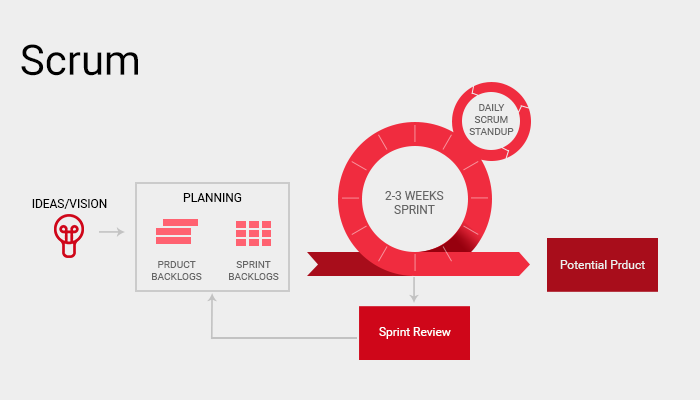
\includegraphics[width=\linewidth]{src/assets/images/ScrumMethodology.png}}
    \caption{ The Agile SCRUM Framework }
    \label{fig:Scrum_Methodology_Diagram}
\end{figure}


% ----------------------------------- SECTIONS (^) ----------------------------------- %
